\documentclass[11pt,a4paper]{article}

% -----------------------------------------------------------------------------
% Paquetes: todos forman parte de una instalacion estandar de LaTeX.
% -----------------------------------------------------------------------------
\usepackage[utf8]{inputenc}
\usepackage[T1]{fontenc}
% Fecha en espanol sin depender de babel ni de spanish.ldf.
\newcommand{\FechaEnEspanol}{%
  \number\day\space de\space
  \ifcase\month
    \or enero\or febrero\or marzo\or abril\or mayo\or junio\or
    julio\or agosto\or septiembre\or octubre\or noviembre\or diciembre
  \fi\space de\space\number\year
}
\usepackage[a4paper,margin=2.5cm,headheight=42pt]{geometry}
\usepackage{graphicx}
\usepackage{xcolor}
\usepackage{fancyhdr}
\usepackage{tikz}

% lastpage no es necesario para compilar, pero permite mostrar "pagina de N".
\newif\ifHayUltimaPagina
\IfFileExists{lastpage.sty}{
  \usepackage{lastpage}
  \HayUltimaPaginatrue
}{
  \HayUltimaPaginafalse
}

% -----------------------------------------------------------------------------
% CONFIGURACION DEL TRABAJO: editar solamente este bloque para reutilizarlo.
% -----------------------------------------------------------------------------
\newcommand{\NombreMateria}{Redes de Computadoras}
\newcommand{\TipoTrabajo}{Trabajo Práctico}
\newcommand{\NumeroTrabajo}{1}
% Cambiar por "Teórico" o "Práctico" según corresponda.
\newcommand{\TipoTP}{Práctico}
\newcommand{\NombreTrabajo}{Comunicaciones 101: Repaso de fundamentos esenciales e introducción a Packet Tracer}
\newcommand{\NombreGrupo}{NetRunners}
\newcommand{\Docente}{SANTIAGO MARTIN HENN}
\newcommand{\LogoArchivo}{logo.png}
\newcommand{\LogoRuta}{\LogoArchivo}

% Una linea por integrante. Se pueden agregar o quitar filas.
\newcommand{\Integrantes}{%
  \begin{tabular}{ll}
    Bastida, Lucas Ramiro & DNI 39444511 \\
    Contessi, Ruben Andres & DNI 33315235 \\
    Garay, Ignacio Hernan & DNI 44191925 \\
    Giraudo, Juan Pablo & DNI 34970089 \\
    Peñaloza, Gonzalo Adrian & DNI 40441355 \\
    Quinteros del Castillo, Tomás Agustín & DNI 46169739 \\
    Vasconsellos Blason, Benjamin Alejandro & DNI 45642879 \\
  \end{tabular}%
}

% -----------------------------------------------------------------------------
% Elementos comunes de caratula y encabezado.
% -----------------------------------------------------------------------------
\newcommand{\InsertarLogo}[1][0.24\textwidth]{%
  \ifx\LogoRuta\empty
    \fbox{\parbox[c][1cm][c]{#1}{\centering Logo institucional\\\small (colocar archivo)}}%
  \else
    \includegraphics[width=#1,keepaspectratio]{\LogoRuta}%
  \fi
}

\newcommand{\TituloCorto}{TP 1 (Práctico): Comunicaciones 101}

\pagestyle{fancy}
\fancyhf{}
\fancyhead[L]{\InsertarLogo[1.4cm]}
\fancyhead[C]{\small\textbf{\TituloCorto}}
\fancyhead[R]{\small\NombreGrupo}
\renewcommand{\headrulewidth}{0.4pt}
\fancyfoot[C]{\small Pagina \thepage\ifHayUltimaPagina\ de \pageref{LastPage}\fi}
\renewcommand{\footrulewidth}{0pt}

\begin{document}

\begin{titlepage}
  \thispagestyle{empty}
  \begin{center}
    \InsertarLogo[0.32\textwidth]

    \vfill
    {\Large\textsc{\NombreMateria}\par}
    \vspace{1.5cm}
    {\Huge\bfseries \TipoTrabajo\par}
    \vspace{0.35cm}
    {\LARGE N.\textsuperscript{o} \NumeroTrabajo (\TipoTP)\par}
    \vspace{0.8cm}
    {\Large\NombreTrabajo\par}

    \vfill
    \begin{tabular}{rl}
      \textbf{Grupo:} & \NombreGrupo \\
      \textbf{Docente:} & \Docente
    \end{tabular}

    \vspace{1cm}
    \begin{center}
      \textbf{Integrantes}\\[0.2cm]
      \Integrantes
    \end{center}

    \vfill
    {\large \FechaEnEspanol\par}
  \end{center}
\end{titlepage}

\section{Objetivos}
\begin{itemize}
  \item Repasar conceptos fundamentales de Comunicaciones. Establecer un vínculo entre la capa física y modelos de transmisión/recepción de datos.
  \item Presentar Packet Tracer, un simulador de redes utilizado para el diseño y análisis de redes de dispositivos.
\end{itemize}

\noindent 3. b).
\begin{figure}[htbp]
  \centering
  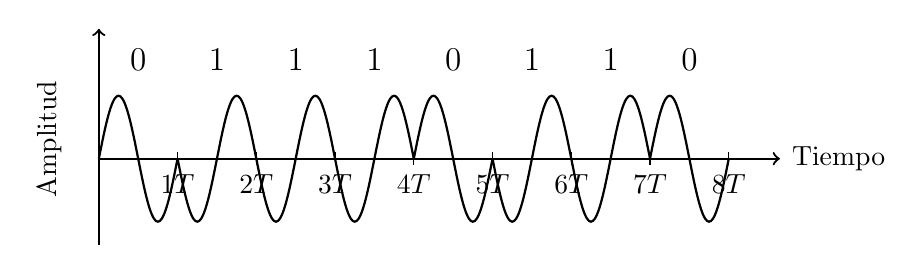
\begin{tikzpicture}[x=1cm,y=1cm]
    \draw[gray!70,densely dotted] (0,0) -- (8,0);

    \foreach \start/\bit in {0/0,1/1,2/1,3/1,4/0,5/1,6/1,7/0} {
      \node[font=\large] at (\start + 0.5,1.25) {\bit};
      \ifnum\bit=0
        \draw[thick,domain=\start:\start+1,samples=41,smooth]
          plot (\x,{0.8*sin(360*(\x-\start))});
      \else
        \draw[thick,domain=\start:\start+1,samples=41,smooth]
          plot (\x,{-0.8*sin(360*(\x-\start))});
      \fi
    }

    \foreach \x in {1,...,8} {
      \draw (\x,0.08) -- (\x,-0.08);
      \node[below] at (\x,-0.08) {$\x T$};
    }

    \draw[->,thick] (0,-1.1) -- (0,1.65);
    \node[rotate=90,anchor=south] at (-0.35,0.25) {Amplitud};
    \draw[->,thick] (0,0) -- (8.65,0);
    \node[anchor=west] at (8.68,0) {Tiempo};
  \end{tikzpicture}
\end{figure}

\end{document}
